\documentclass{article}

\usepackage{graphicx}
\usepackage{cleveref}
\usepackage{listings}
\usepackage{booktabs}

\usepackage[vmargin=2.2cm]{geometry}

\usepackage[T1]{fontenc}
\usepackage[utf8]{inputenc}
\usepackage{helvet}
\renewcommand{\familydefault}{\sfdefault}

\usepackage{harvard}
\usepackage{bibgerm}

\title{Pfad Planung A* vs ROS nativ}
\date{2020 Juni}
\author{Jonathan König}

\begin{document}

\maketitle
\newpage

\tableofcontents

\newpage
\clearpage
\pagenumbering{arabic}



\section{Aufgabenstellung}

\begin{figure}[!htbp]
    \centering
    
\includegraphics[width=0.5\linewidth]{../src/koenig/maps/bmrMap.png}
    \caption{Maze}\label{map}
\end{figure}

Problemstellung der Aufgabe ist die Pfadplanung. Diese sollte auf zwei verschiedene Arten gelöst werden. Einerseits durch die in ROS native Pfadplanung, andererseits durch einen selbst implementierten Algorithmus.
Gegeben ist eine Karte (siehe Abbildung \ref{map}), in der vom linken unteren Eingang zum rechten oberen Ausgang navigiert werden soll.

Es wurden zwei Lösungen implementiert:
\begin{enumerate}
    \item Pfadplanung durch den ROS nativen NavfnROS Planer
    \item Pfadplanung durch Implementierung des A* Algorithmus 
\end{enumerate}

\section{DWAPlannerROS }
\label{DWAPlannerROS}

Das Ziel wird via einer eigens geschriebenen Publisher Node \verb|goal_pub| in x- und y-Koordinaten über einen Action Client an die \verb|move_base| Node übergeben.
Die Node \verb|move_base| holt sich über die Nodes \verb|joint_state_publisher| und \verb|robot_state_publisher| die Daten zum turtlebot burger. Die Node \verb|tf| bestimmt in welcher Startposition sich der Roboter und somit der Ausgangspunkt der Pfadplanung befinden.

Der DWAPlannerROS verwendet den sogenannten Dijkstra Algorithmus, um den kürzest und schnellst möglichen Pfad zu errechnen. Hierbei wird jede mögliche Position als eigener Knoten betrachtet. Der Start-Knoten stellt die Anfangsposition, und der End-Knoten die gewünschte Endposition dar. Um nun den kürzesten Weg auszurechnen, wird anhand von Kosten, die durch \verb|costmaps| ermittelt werden, abgewägt welcher Knoten als nächstes angefahren werden soll. Dies wird solange getan bis der gewünschte End-Knoten erreich ist. 

Sobald der DWAPlannerROS den kürzesten Pfad ermittelt hat, wird dieser an die Node \verb|move_base| übergeben, welche den Pfad folglich published (siehe Abbildung \ref{path_nativ}).

\begin{figure}[!htbp]
    \centering
    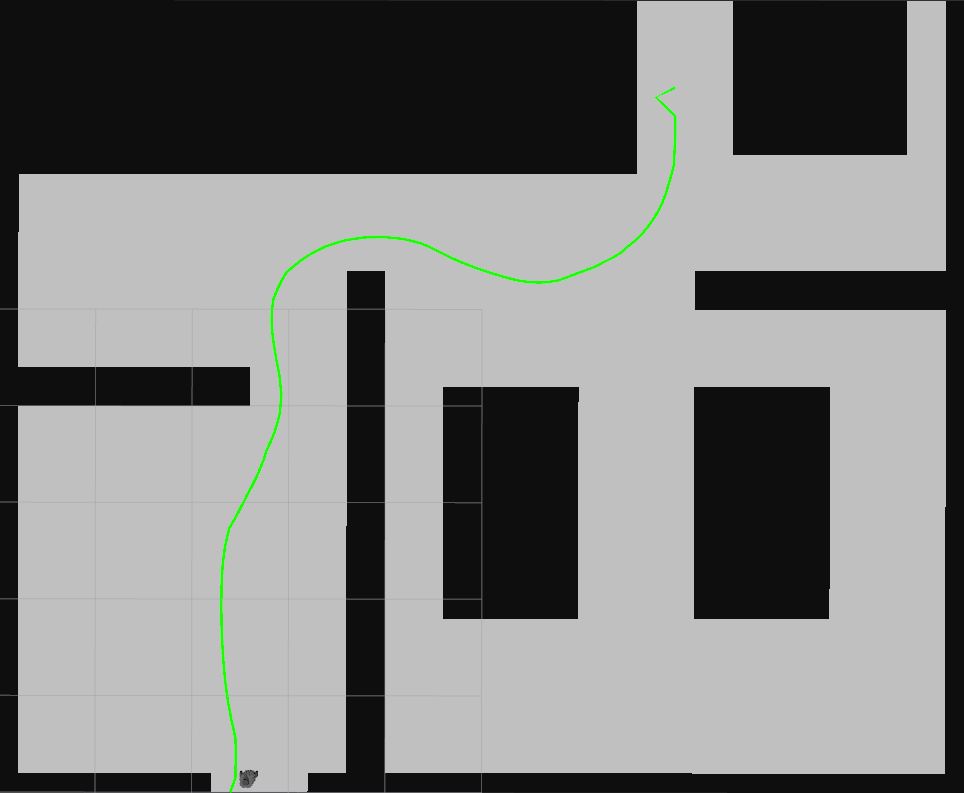
\includegraphics[width=0.5\linewidth]{PICs/nativ_rviz_plan.png}
    \caption{Native Pfad}\label{path_nativ}
\end{figure}

\section{Custom Path Planner}

Die selbst konzipierte Lösung zur Pfadfindung wurde realisiert, indem die Node \verb|finder| geschrieben wurde, in welcher der A* Algorithmus implementiert ist.

Der A* Algorithmus operiert ähnlich wie Dijkstra, jedoch erweitert er diesen um eine Schätzfunktion, die sogenannte Heuristik. Hierbei werden die Kosten des bisher zurückgelegten Weges mit einem Schätzwert der Distanz zum Ziel-Knoten addiert, was dann die geschätzten Gesamtkosten ergibt. 

Optimierungspotential gibt es diesem Fall bei der gechätzten Distanz zum Ziel durch den Satz von Pythagoras, welche Wände ignoriert. Weiters kann die Pfadplanung weiter durch die Bestimmung der Höhe der Kosten verbessert werden.

Um die Node \verb|goal_pub| weiter verwenden zu können ist in der Node \verb|finder| ein Action Server intergriert, um die Node \verb|goal_pub| weiter verwenden zu können. Hierfür war es nötig eine Klasse \texttt{pixel} zu erstellen, welche Attribute für jedes Raster Teil der Karte beinhaltet.

\begin{lstlisting}
class pixel{
    public:
        bool is_obstical;
        pair<int, int> parents, location;
        double goal_distance;
        double walked_distance, heuristik;

        pixel();
};
\end{lstlisting}

Bevor begonnen wird zu suchen wird für jedes Pixel die \verb|location| und die \verb|goal_distance| gesetzt. 
Daraufhin wird der A* Algorithmus für die Start und Ziel Position durchgeführt und der Pfad gepublished, siehe \ref{path_custom}.

\begin{figure}[!htbp]
    \centering
    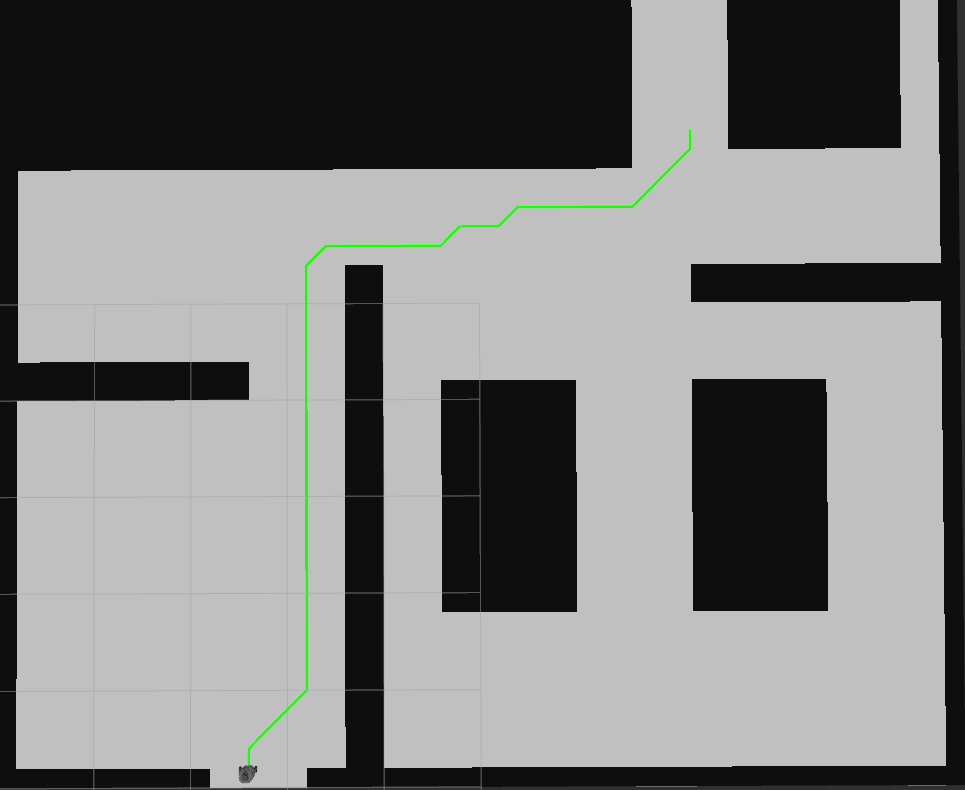
\includegraphics[width=0.5\linewidth]{PICs/custom_rviz_plan.png}
    \caption{Custom Pfad}\label{path_custom}
\end{figure}

\section{Vergleich der beiden Lösungen}

\textbf{Completeness}\newline

Beide Algorithmen finden in diesem Szenario eine Lösung, die sie an das angegebene Ziel führt. 

\begin{table}[!htbp]
    \begin{tabular}{p{7cm}|p{7cm}}
        DWAPlannerROS & custom A Star \\ \bottomrule
        Lösung vorhanedn & Lösung vorhanedn
    \end{tabular}
\end{table}

\textbf{Optimality}\newline

A* ist findet generell den optimaleren Pfad, aufgrund der angewandten Heuristik. Unterschiedliche Pfade können mit Veränderung der Bewertung von Kosten gefunden werden. Somit hat man mehr Optimierungspotential als beim Dijkstra Algorithmus.

\begin{table}[!htbp]
    \begin{tabular}{p{7cm}|p{7cm}}
        DWAPlannerROS & custom A Star \\ \bottomrule
     berücksichtigt das der Roboter nicht unendlich schnell sich drehen kann & Sollte den kürzesten Pfad finden doch nur mit 45 pfaden möglich
    \end{tabular}
\end{table}


\textbf{Time complexity}\newline

Die Zeitintensivität der beiden Algorithmen an diesem Beispiel zu vergleichen ist schwierig da der native DWAPlannerROS Pfadplaner diverse Optimierungsmöglichkeiten hat, welche in dem selbst konzipierten A* fehlen.
Generell kann man jedoch behaupten, dass A* schneller ist, da wesentlich weniger Knoten bearbeitet werden.

\begin{table}[!htbp]
    \begin{tabular}{p{7cm}|p{7cm}}
        DWAPlannerROS & custom A Star \\ \bottomrule
    langsamer & schneller als Dikstra weil weniger Knoten durchsucht werden müssen aufgrund der Heristik
    \end{tabular}
\end{table}

\textbf{Space complexity}\newline

Dijkstra ist A* überlegen, wenn es mehr als ein Ziel gibt, da er die Distanzen vom Startpunkt zu einem wesentlich größeren Teil des Graphen ausrechnet, während A* stets zu einem vordefinierten Ziel führt.

\begin{table}[!htbp]
    \begin{tabular}{p{7cm}|p{7cm}}
        DWAPlannerROS & custom A Star \\ \bottomrule
        test & some
    \end{tabular}
\end{table}

https://www.slant.co/versus/11584/11585/~dijkstra-s-algorithm_vs_a-algorithm

\end{document}
